\chapter{Background Survey}
\label{backgrnd}
There have been many projects and programs created to try to tackle to complexities of managing \bibtex{} entries, some of which will be examined herein.  Firstly, some of the criteria for examinations are listed, before discussing the examinations and then a summary of findings of the examinations are presented, to be kept in mind during the rest of the project.

The products that are examined are:
\begin{enumerate}
	\item \bibtex{} Entry Manager by Ravi Tez Kota
	\item BiblioScape by CG Information
	\item \bibtex{} Manager by Mitesh Pravin Furia 
\end{enumerate}

\section{Examination Criteria}
The products examined in this section will be judged on several factors, outlined below.

Each assessment will examine how positive qualities are achieved, as well as how shortcomings are encountered, so that lessons can be learned from other products and problematic issues can be avoided.  It is advantageous at this point to mention that evaluations on the final product from this project will include an examination on the same criteria in Chapter~\ref{eval}.
\begin{enumerate}
	\item \gls{ui} to the system:
	\begin{enumerate}
		\item How well laid out is the \gls{ui}? 
		\item Is it consistent throughout use?
		\item Is it cluttered and complicated or well spaced out and simple?
		\item Is it intuitive to deduce how a user should perform an action and, where it is not, is it easy to get help?
		\item Is it clear when an action has been performed?
		\item Does it have a look and feel that is easy on the user's eyes?
	\end{enumerate}
	\item Features of the system:
	\begin{enumerate}
		\item Does the system support multiple users? If so, how?
		\item What expected and basic\footnote{`Basic' functions are defined to be Add, Edit, Delete, Import, Export and Search. These functions were designated `basic' after developing a general understanding of what a reference management system is expected to do at early project meetings with Dr Manlove.} functions are available for the user to perform? Are any missing?  % acceptable?
		\item What further\footnote{`Further' functions are defined to be any function other than those mentioned in footnote 1 (Add, Edit, Delete, and so on.)} functions are available to the user? 
		\item What range of formats are available to import from and export to?
		\item How well documented is the system?
	\end{enumerate}
	\item Fault Tolerance/Robustness:
	\begin{enumerate}
		\item How well does the program cope with poorly formatted entries?
		\item How well does the program cope with invalid user input?
		\item Is the software free from visible errors and problems?
	\end{enumerate}
\end{enumerate}

\section{Examinations}
This section contains the examinations of several existing products, both public projects and previous projects undertaken by students in previous years at the University of Glasgow.  Examinations were performed on a laptop running Windows 7 Professional (64-bit edition).

\subsection{\bibtex{} Entry Manager}
The \bibtex{} Entry Manager was developed by Ravi Tez Kota, an M.Sc. student at the University of Glasgow, under Dr Manlove's supervision in 2010.

\subsubsection{Paradigm}
This project is a web-based reference management system which consists of a database for storage of entries and a web front-end for users to interact with using a web browser.

\subsubsection{Ease of set-up}
In a nutshell, the server side of the product is not convenient to set-up.  The user must have an instance of MySql server running on the machine from which they'd like to serve pages; they must ensure that Apache Tomcat is installed as a page rendering server; and they must have a \gls{jre} installed.  The installers for each of these products were included with the content of the product, though that did not greatly reduce the effort required to set them up.  Following set-up of software components, the user must set up the database using a provided \gls{sql} script and finally add the `bibtex' directory to Apache Tomcat's content directory.  

This may be a lengthy process, but it only has to be done once per instance of the system, which works in its favour. If the system were set up at a central location, many people could log on to the system at once by visiting a \gls{url}, which would give end-users a very simple method of access without involving them in the set up process (as is intended with a web-based product).

\subsubsection{Examination of product}
After installation, the program is easy to navigate to; the user simply points their web browser to the \gls{url} and the initial page is loaded. The system supports different users by way of a registration and log-in process, authenticated with a user name (email address) and password combination.

The sign-up and log-in pages are simple and consistent in terms of layout, but after logging in the look and feel of the site changes (see figure \ref{fig:RaviLoginScreen} and figure \ref{fig:RaviListScreen}).  This is useful in terms of letting the user know that they are authenticated, but it means that one must re-acquaint oneself with the new layout before performing any actions.  Reducing this extra burden in terms of cognitive load would be advantageous in a new system.


\begin{figure}
	\begin{center}
		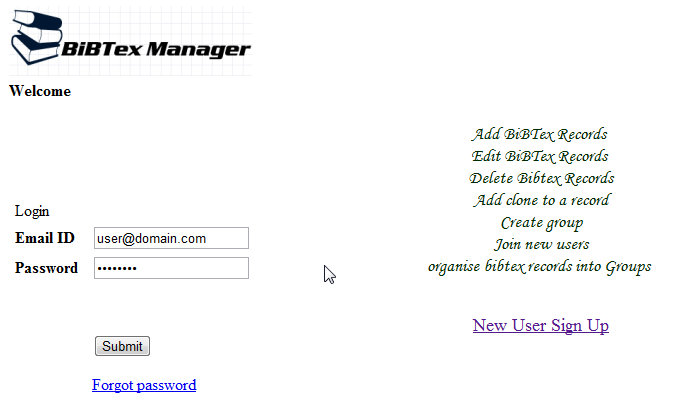
\includegraphics
			[scale=0.65]
			{images/LoginScreen.png}
		\caption{BibTeX Entry Manager Login Screen}
		\label{fig:RaviLoginScreen}
	\end{center}
\end{figure}

\begin{figure}
	\begin{center}
		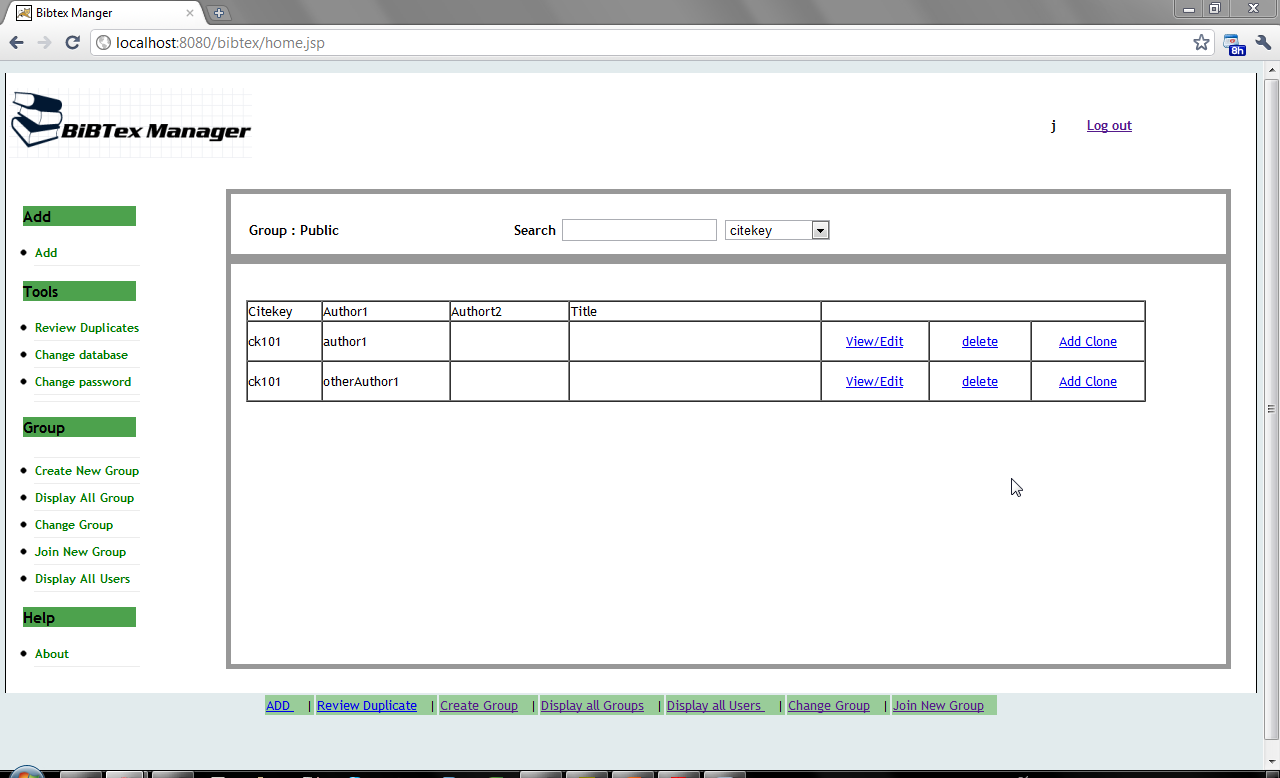
\includegraphics
			[scale=0.4]
			{images/RaviListScreen.png}
		\caption{BibTeX Entry Manager List Entries Screen}
		\label{fig:RaviListScreen}
	\end{center}
\end{figure}

The product has two navigation areas which contain different sets of commands in different orders. 
In setting out to perform this background research, it was intended that the examiner would upload/open a file and perform further additions, modifications, deletions and searches across known entries from that initial file.  The lack of file import capability in the product was somewhat limiting to the consistency of the examination on this product, and was a significant shortcoming of the product. 

It is easy to deduce from the homepage what a user should click to add an entry to the system, though after an addition is performed, no message is shown to indicate success or failure of the operation.  It is clear that Nielsen's first heuristic \cite{NielsenHeuristics}\footnote{\label{nielsenH1} Nielsen's first heuristic says that the system should always keep users informed about what is going on. (Visibility of system status)} should be adhered to when designing future solutions to this problem.% don't think it is sufficient just to cite this web page, though they are listed here: http://www.useit.com/papers/heuristic/heuristic_list.html

After a break of perhaps twenty minutes in the examination, the user returned and reloaded the home page of the project, only to find that an error had occurred (a NullPointerException was thrown, resulting in a \gls{http} 500 error).  The error was not dealt with in a user-friendly fashion and shows the product in an unprofessional light.  The lesson to be learned here is that the product should deal with errors in a professional manner and not show exceptions on screen to users.

There is no provided `export' functionality, so items cannot be taken out of the system and used directly in the \bibtex{} environment without first reconstructing the entry.  This is quite inconvenient for a user; the lesson to be learned from this is that basic functionality should be provided to ensure that the system is useful to a user.
The modification of an entry is relatively straightforward, although if a user wishes to change an entry's type after it has been saved to the database they will be disappointed, as the entry type is not a field that can be changed by any visible means without re-creating it in the database: users should be able to change an entry's type at any point after creation.

Searching is a bit of a mystery with this product; it is difficult to deduce what state a search is in, given that there is no feedback to the user to say that a search is ongoing, complete, or otherwise.  This lack of feedback makes for a confusing experience with search and adds to the call for future projects and solutions to adhere to Nielsen's first heuristic. Unfortunately, there is no visible help menu or area to the product to help to describe how any of the functions behave, which is something that would have been particularly helpful to assist with the search function, which is another concern that Nielsen addresses in his list of heuristics.  This lack of help or support is a shortcoming of the product and future projects should provide to avoid usability issues.

There is a provision for users to be able to switch to another database server from the one that they are using.  This might be helpful to some users, but there is potential for unnecessary replication across multiple servers.  It is also unclear from the user interface what database engines and schemas are supported by the system, which is another point that should be well covered by a user manual or help system.

Entries can be categorised by users into different groups and allows a user to choose between groups currently in view \ref{fig:ChangeGroupScreen}.  This involves creating a group with a name and a description, changing to the new group and then adding entries to the group by the method previously used.  This is a helpful feature for categorising entries that do not yet exist, but a limitation of the system is that entries cannot be transferred from one group to another, and it means that they cannot belong to more than one group at any time.  Any future system implementing a grouping capability should allow entries to belong to many groups and should allow modification at any stage after addition to the set of entries, rather than restricting the flexibility of the system by failing to provide the functionality to make these changes.

\begin{figure}
	\begin{center}
		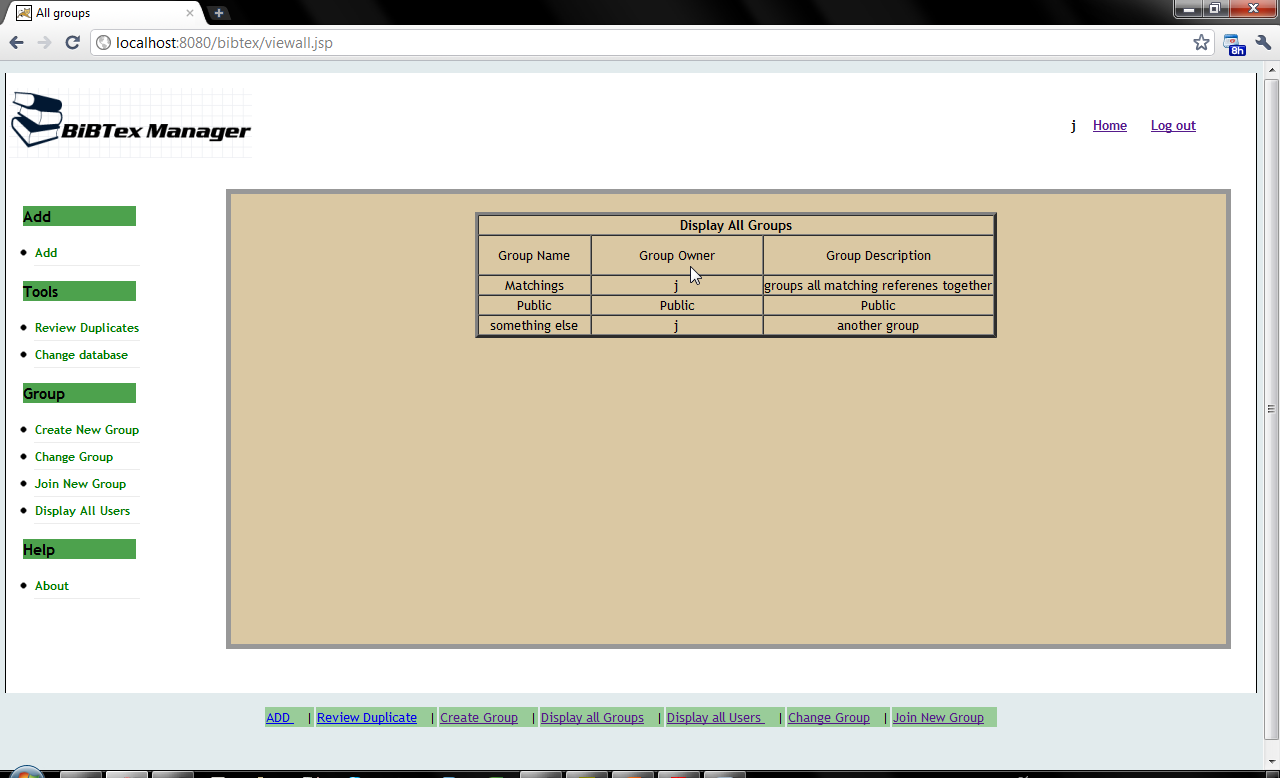
\includegraphics
			[scale=0.4]
			{images/ChangeGroupScreen.png}
		\caption{BibTeX Entry Manager Change Group Screen}
		\label{fig:ChangeGroupScreen}
	\end{center}
\end{figure}

The site allows users to access the same set of entries at the same time.  An issue that arises from this is that users may make changes to the same entry simultaneously, which could leave the entries in an inconsistent or incorrect state.  The solution deals with the problem by locking an entry until the first user to access it saves any changes they have made, or exits the viewing window.  This solution means that there can be absolutely no overlapping of interests when multiple people access the same entry.  An issue that arises from this method, however, is that if one user (user A) views an entry, then forgets to close the window, the entry is locked for a period of time.  When users B and C come to view it (perhaps with no intention of modifying it), they find that they cannot access it (see figure \ref{fig:RaviEditing}, leaving them unable to work and potentially frustrated while user A's time period of user A's viewing expires.  The system works on a pessimistic concurrency approach --- one that works on the assumption that clashes occur frequently --- and utilises a solution similar to the `locking' version control strategy.  This pessimistic strategy might not be optimal for the application and other approaches should be examined for future systems.

\begin{figure}
	\begin{center}
		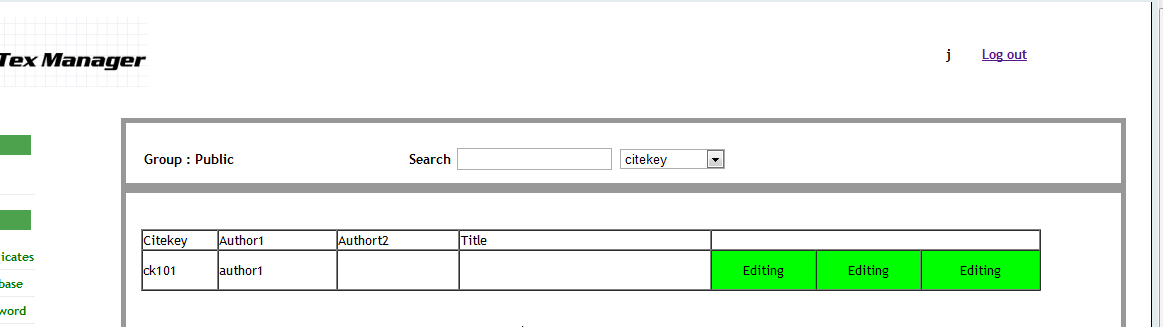
\includegraphics
			[scale=0.45]
			{images/RaviEditing.png}
		\caption{BibTeX Entry Manager -- Editing Notification}
		\label{fig:RaviEditing}
	\end{center}
\end{figure}


\subsection{BiblioScape}
BiblioScape is a desktop-based bibliographic data and note collection suite produced by CG Information.  It was created with the aim to ``build first class bibliographic software for the 21st century''.  It contains many tools which shall not be included in this examination as they are deemed to be surplus to requirements for the scope of the current project.\footnote{The system includes a forum and task list, among other things.} The live demo system is not as up to date as its current desktop counterpart (pictured on the website running on Windows 7), as the copyright notice at the foot of the home page dates back to 2002, where Windows 7 was released to the public in 2009 \cite{Win7Release}.

\subsubsection{Paradigm}
As part of the BiblioScape package, `BiblioWeb' was produced to ``address the needs of researchers in the age of the Internet'' \cite{BiblioWebWhy}.  It is a web-based version of their desktop program and allows users to access it through internet and Intranet connections.

\subsubsection{Ease of set-up}
A live version of the product was used on the BiblioScape website\footnote{The live version of the website is hosted at http://support.biblioscape.com:8001/}, so no comment can be made on the set-up process.

\subsubsection{Examination of product}
BiblioWeb has a clean \gls{ui}, and boasts a consistent navigation area at the top, whether a user is logged in or not.  Items in the menu at the top are spaced far enough apart that the interface feels uncluttered while also providing most of the basic options that a user expects of a reference management system, although edit, delete and export are not immediately apparent from the navigation bar, as can be seen in figure \ref{fig:BiblioScapeHomePage}. 

\begin{figure}
	\begin{center}
		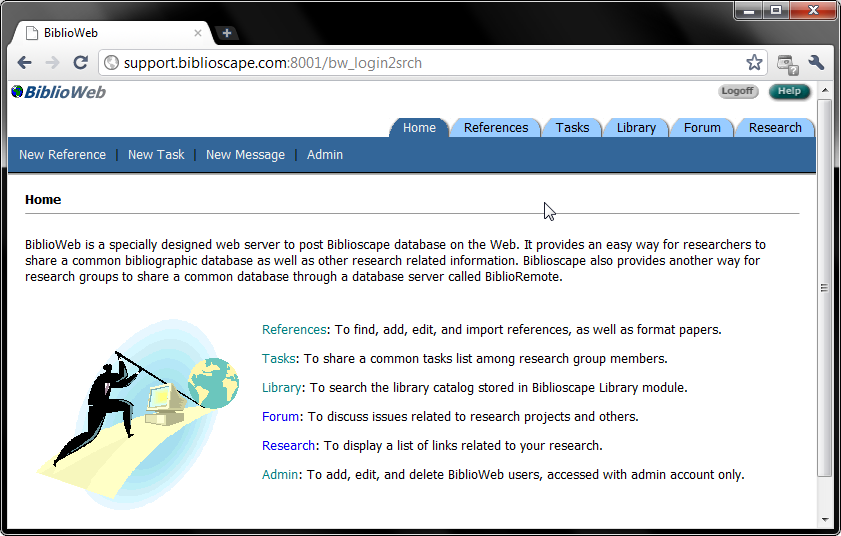
\includegraphics
			[scale=0.65]
			{images/BiblioScapeHomePage.png}
		\caption{BiblioScape Home Page (immediately after log-in)}
		\label{fig:BiblioScapeHomePage}
	\end{center}
\end{figure}

It has an intuitive interface and makes it quite clear where one should go next when performing tasks.  One cannot obtain a list of all entries in the system, which means that a user might be forced to recall all information about an entry rather than rely on recognition; Nielsen \cite{NielsenHeuristics} specifies a heuristic guideline (his sixth out of ten) that a user's memory load should be minimised by making objects, actions and options visible.

BiblioWeb allows categorisation of references by use of folders (see figure \ref{fig:BiblioScapeFolderView}), much like the grouping function in the first project.  Some advantages that BiblioWeb's grouping method has over the first project's method include firstly that one can move many references at once from one categorisation to another, and secondly there is no need to delete an entry before reclassifying it.  It does appear, however, that references can only be in one folder at a time, which limits the flexibility of entries and perhaps allows redundancy in the database, where it could have been avoided by allowing an entry to belong to more than one category. 

\begin{figure}
	\begin{center}
		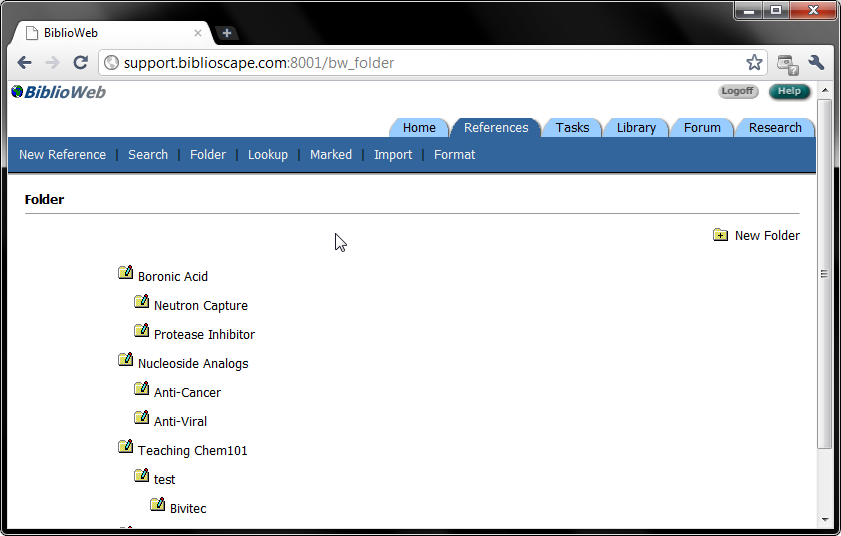
\includegraphics
			[scale=0.65]
			{images/BiblioScapeFolderView.png}
		\caption{BiblioScape Folder View}
		\label{fig:BiblioScapeFolderView}
	\end{center}
\end{figure}

Users' actions are clearly indicated when they are completed successfully, but the system falls down when incorrect input is supplied.  An example of this is explained presently: text was supplied to the `year' field to see how the system behaved with a string supplied instead of an integer.  Rather than displaying a helpful error message on the interface, the system navigated to a plain white page and displayed the word `EXCEPTION', followed by what is presumably a database exception.  As was the case in the first solution, the system did not handle errors and exceptions in a user-friendly way.  It is important to ensure that the system deals with problems in a professional and informative manner, so that a user can recover from their error --- something that Nielsen covers in his list of heuristics \cite{NielsenHeuristics}.

Perhaps the greatest asset of the BiblioWeb system has is its import function which boasts an enormous list of text and file formats, as can be seen in figure \ref{fig:BiblioScapeImportScreen}.  There are unfortunately not enough resources for this experiment to test all 201 of the formats, but it is safe to say that the system handles parsing of \bibtex{} entries well.  The system does not store the entries' types as would be expected of a \bibtex{} reference management package: rather than storing the reference type `Unpublished' as it was in the \bibtex{} file, it stored `Personal Communication', which is not accurate to the \bibtex{} format, and subsequently leaves the terminology open to misinterpretation by a user.

\begin{figure}
	\begin{center}
		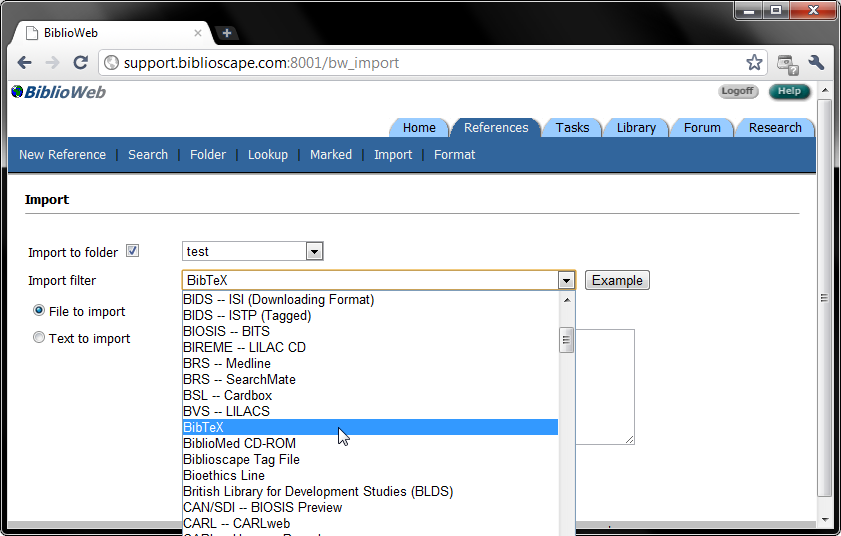
\includegraphics
			[scale=0.65]
			{images/BiblioScapeImportScreen.png}
		\caption{BiblioScape Import Page}
		\label{fig:BiblioScapeImportScreen}
	\end{center}
\end{figure}

The system's single greatest failure is that it does not support the export of entries to the \bibtex{} format.  This is a fatal flaw in terms of using the product with the main intended package of the project, \bibtex, although it does export to BiblioScape tag file, EndNote, RIS and Unix Refer formats, so can be used with their respective packages.


\subsection{\bibtex{} Manager}
\bibtex{} Manager is a reference manager specifically created for management of \bibtex{} entries.  It was written in Java by Mitesh Pravin Furia during 2009 as part of the requirements of the MSc IT degree at the University of Glasgow.

\subsubsection{Paradigm}
The product is a desktop-based application which can connect to a database, presumably to allow concurrent and multi-user access, though no user manual is included and it was not possible to test the feature.

\subsubsection{Ease of set-up}
The product was very easy to set up; it simply requires that a \gls{jre} is installed, which is obtainable from \url{http://www.java.com}.

\subsubsection{Examination of product}
The \gls{ui} to the system is well laid out and well spaced out. The application follows the convention of many desktop-based applications and uses a menu bar at the top, containing the `File' menu, along with `Edit', `Tools' and `About'.  The menus remain consistent throughout use and are a solid go-to point for most pieces of functionality, which works well in the application's favour.

It does not appear that multi-user access is supported by the program; there is no option to log in as a user

The consistent menu is complimented by a consistent table area where currently loaded entries are displayed.  It is clear when there are no entries, as the area is greyed out slightly and the presence of entries in the system is also clear, thanks to the display of each entry as a row in the table.  An entry is selected by clicking on it, though it does not encourage a user to click by appearing to be clickable, as it has been styled to look like a display table  \revisit HCI affordance notes.

The program deals with correct input successfully, and does not have any difficulty parsing correctly formatted files.  It gives some feedback for successful cases, though it would be helpful to know how many entries were successfully imported. 

A problem arises when there is incorrect user input or an erroneous entry is passed to the system; when adding or modifying an entry, it is possible to submit and save an entry with some of the `required' fields left incomplete.  This would not be such a problem if the interface had some way of marking invalid entries, but entries can be stored and exported to a file with no warning to the user that any invalid entry was encountered; a problem that has the potential to cause errors and problems when the exported file is used with \bibtex{}.

\revisit{} --- More to come.
\revisit{} --- More to come.
\revisit{} --- More to come.

% one per product
%\subsection{Product name}
%\subsubsection{Paradigm}
%\subsubsection{Ease of set-up}
%\subsubsection{Examination of product}
%content

\section{Summary}
A summary of lessons learned from these examinations is listed presently:
\begin{enumerate}
	\item Make it easy for a user to set up, where possible.
	\item provide feedback to users when actions have occurred 
	\item Keep errors under wraps where possible and deal with them neatly otherwise.
	\item groups: allow groups to change for existing entries and let entries change groups after initial storage
	\item control access to entries in a way that does not impede the progress of other users.
	\item Keep pages consistent to reduce cognitive load on a user.
	\item Support \bibtex{} import and export.
	\item make it easy to navigate to
	\item basic functionality should be provided to ensure that the system is useful to a user
	\item users should be able to change an entry's type at any point
	\item other concurrent access approaches should be examined for future systems
	\item 
	\item \revisit --- All lessons learned will be enumerated here.
	\item 
\end{enumerate}

These lessons should be kept in mind when creating requirements, designing the solution and during implementation of the software.